% !TeX program = pdflatex
% !TeX encoding = UTF-8
% -----------------------------------------------------------------------------
% Generic Taylor & Francis / Routledge journal-article manuscript
% -----------------------------------------------------------------------------
% Taylor & Francis journals do not all use the same LaTeX class. Before
% submission, check the target journal's Instructions for Authors and replace
% this preamble with a journal-specific class if one is supplied. This portable
% version follows the publisher's general manuscript advice: 12-point Times,
% double spacing, and margins of at least 2.5 cm. It is intentionally
% self-contained: figures, tables, and references all compile from this file.
%
% To prepare a clean reading copy, change \reviewtrue to \reviewfalse below.

\documentclass[12pt,a4paper]{article}

% --- Encoding and typography -------------------------------------------------
\usepackage[T1]{fontenc}
\usepackage[utf8]{inputenc}
\usepackage{amsmath,amssymb}
\usepackage{newtxtext,newtxmath}
\usepackage{microtype}
\usepackage[a4paper,margin=2.5cm]{geometry}
\usepackage{setspace}

% --- Mathematics, tables, and figures ---------------------------------------
\usepackage{booktabs}
\usepackage{tabularx}
\usepackage{array}
\usepackage{graphicx}
\usepackage{caption}
\usepackage{siunitx}
\usepackage{tikz}
\usetikzlibrary{arrows.meta,positioning}
\usepackage{pgfplots}
\pgfplotsset{compat=1.18}

% --- Front matter, citations, and review aids -------------------------------
\usepackage{authblk}
\usepackage[authoryear,round]{natbib}
\usepackage[switch]{lineno}
\usepackage{enumitem}
\usepackage{xcolor}
\usepackage[hidelinks]{hyperref}

\definecolor{tandfblue}{HTML}{1F4E79}
\definecolor{tandfteal}{HTML}{2A7F86}
\definecolor{tandfgold}{HTML}{C58A1C}

\captionsetup{font=small,labelfont=bf,labelsep=period}
\setlist{itemsep=0.25em,topsep=0.5em}
\sisetup{detect-all,round-mode=places,round-precision=1}
\renewcommand{\Authfont}{\normalsize}
\renewcommand{\Affilfont}{\small\itshape}
\renewcommand{\Authands}{ and }

% --- Review / reading-copy switch -------------------------------------------
\newif\ifreview
\reviewtrue
\ifreview
  \doublespacing
\else
  \setstretch{1.15}
\fi

% --- Reusable metadata -------------------------------------------------------
\newcommand{\articletype}{Original Article}
\newcommand{\shorttitle}{Robust computational research pipelines}
\newcommand{\correspondingemail}{maya.chen@example.edu}

\hypersetup{
  pdftitle={A robustness-first framework for reproducible computational research pipelines},
  pdfauthor={Maya Chen, Daniel Okafor, and Sofia Alvarez},
  pdfsubject={Example Taylor and Francis journal article manuscript},
  pdfkeywords={computational reproducibility, dependency management, open science,
    robustness, simulation study}
}

\title{A robustness-first framework for reproducible computational research
  pipelines: a simulation study}

\author[1]{Maya Chen\thanks{Corresponding author: \href{mailto:\correspondingemail}{\correspondingemail}}}
\author[2]{Daniel Okafor}
\author[1,3]{Sofia Alvarez}
\affil[1]{Centre for Open Methods, Northbridge University, Northbridge, UK}
\affil[2]{Department of Statistics, Lakeview Institute of Technology, Toronto, Canada}
\affil[3]{Research Software Group, Instituto del Pacifico, Valparaiso, Chile}

\date{}

\begin{document}

\maketitle

\begin{center}
  \small\textbf{Article type:} \articletype
\end{center}

\begin{abstract}
Computational results may fail to reproduce when software dependencies,
execution environments, or random processes are incompletely specified. We
developed a robustness-first framework that evaluates a research pipeline under
controlled environmental perturbations rather than testing it only in its
original environment. A simulation study compared three documentation
strategies---fully pinned, partially specified, and unpinned---across 300
synthetic analysis projects and 100 perturbed rebuilds per project. The primary
outcomes were successful execution and numerical deviation from a reference
result. Fully pinned projects reproduced successfully in 96.7\% of rebuilds,
compared with 82.4\% for partially specified projects and 61.3\% for unpinned
projects. Environment capture reduced numerical deviation, while explicit
random seeds chiefly reduced variation among successful runs. These effects
were complementary rather than interchangeable. The framework turns
reproducibility from a one-time claim into a measurable stress test and provides
a concise reporting structure for authors, reviewers, and research-software
teams. The study is illustrative, but the workflow can be adapted to empirical
pipelines in any computational discipline.
\end{abstract}

\noindent\textbf{Keywords:} computational reproducibility; dependency
management; open science; robustness; simulation study

\vspace{0.75\baselineskip}
\noindent\textbf{Subject classification codes:} 68N30; 62J05

\ifreview
  \linenumbers
\fi

\section{Introduction}

Reproducibility is a foundation of cumulative computational research, yet the
term describes several distinct goals. A result may be repeatable in the
original environment, reproducible from shared code and data, or robust to
reasonable changes in software and hardware. Treating these goals as a single
binary property can conceal important failure modes \citep{peng2011,stodden2016}.
For example, a script may execute today but fail after an indirect library is
updated, or it may run successfully while producing a materially different
estimate because a random seed was not recorded.

Practical guidance emphasizes version control, scripted analyses, preserved raw
data, and recorded intermediate results \citep{sandve2013}. The FAIR principles
similarly stress that digital research objects should be findable, accessible,
interoperable, and reusable \citep{wilkinson2016}. These practices improve the
conditions for reuse, but they do not by themselves quantify how resilient a
pipeline is to environmental change. A robustness test is therefore a useful
companion to a reproducibility checklist.

This study presents a small, transparent framework for stress-testing
computational pipelines. We ask three questions:

\begin{enumerate}
  \item How strongly does dependency specification affect execution success?
  \item Do environment capture and random-seed control address the same failure
        mode or complementary ones?
  \item Which compact set of measures communicates pipeline robustness without
        obscuring the underlying failure mechanisms?
\end{enumerate}

The resulting manuscript also demonstrates the expected structure of a general
Taylor \& Francis submission, including author affiliations, an abstract,
keywords, equations, figures, tables, data and code statements, contributor
roles, disclosure, funding, and an author--date reference list.

\section{Methods}

\subsection{Study design}

We generated 300 synthetic analysis projects, each representing a common
read--transform--model--report workflow. Every project contained a tabular input,
a deterministic preprocessing stage, a regression model, and a rendered summary
report. Projects were allocated equally to three environment-documentation
strategies:

\begin{description}[style=nextline]
  \item[Fully pinned]
  Direct and transitive dependency versions, operating-system metadata, and a
  cryptographic lock file were recorded.

  \item[Partially specified]
  Direct dependencies and their minimum versions were recorded, but transitive
  versions and system libraries were allowed to vary.

  \item[Unpinned]
  Package names were recorded without version constraints; the most recent
  compatible packages were selected at rebuild time.
\end{description}

Each project was rebuilt 100 times under perturbations representing dependency
updates, changes in system libraries, and processor-level numerical variation.
Half of the projects in each strategy recorded an explicit random seed. The
simulation therefore contained 30,000 rebuild attempts. Figure~\ref{fig:workflow}
summarizes the design.

\begin{figure}[tbp]
  \centering
  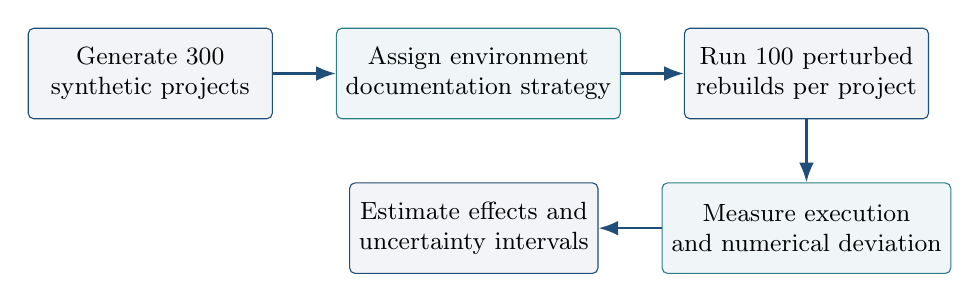
\begin{tikzpicture}[
    node distance=8mm and 8mm,
    box/.style={draw=tandfblue,rounded corners=2pt,fill=tandfblue!6,
      minimum width=3.1cm,minimum height=1.15cm,align=center,font=\small},
    decision/.style={draw=tandfteal,rounded corners=2pt,fill=tandfteal!7,
      minimum width=3.1cm,minimum height=1.15cm,align=center,font=\small},
    arrow/.style={-{Latex[length=2.5mm]},thick,tandfblue}
  ]
    \node[box] (projects) {Generate 300\\synthetic projects};
    \node[decision,right=of projects] (strategy) {Assign environment\\documentation strategy};
    \node[box,right=of strategy] (rebuild) {Run 100 perturbed\\rebuilds per project};
    \node[decision,below=of rebuild] (measure) {Measure execution\\and numerical deviation};
    \node[box,left=of measure] (compare) {Estimate effects and\\uncertainty intervals};
    \draw[arrow] (projects) -- (strategy);
    \draw[arrow] (strategy) -- (rebuild);
    \draw[arrow] (rebuild) -- (measure);
    \draw[arrow] (measure) -- (compare);
  \end{tikzpicture}
  \caption{Robustness-testing workflow used in the simulation study. Every
  synthetic project was evaluated repeatedly under controlled environmental
  perturbations.}
  \label{fig:workflow}
\end{figure}

\subsection{Outcomes}

The primary binary outcome, execution success, indicated that the pipeline
completed and produced every declared output. For successful rebuilds, numerical
deviation measured the scaled absolute difference between a rebuilt estimate
$\hat{\theta}_{ir}$ and the project's reference estimate $\hat{\theta}_{i0}$:

\begin{equation}
  d_{ir} =
  \frac{\left|\hat{\theta}_{ir}-\hat{\theta}_{i0}\right|}
       {\max\!\left(\left|\hat{\theta}_{i0}\right|,\epsilon\right)},
  \qquad \epsilon = 10^{-8},
  \label{eq:deviation}
\end{equation}

where $i$ indexes projects and $r$ indexes rebuilds. We report $100d_{ir}$ as a
percentage. A rebuild was classified as substantively reproduced when it both
executed successfully and had $d_{ir}<0.01$.

\subsection{Statistical analysis}

Execution success was summarized by strategy with project-clustered bootstrap
intervals based on 2,000 resamples. A logistic regression estimated contrasts
between documentation strategies. Among successful rebuilds, a log-linear model
estimated associations between numerical deviation, environment strategy, and
seed control. We included their interaction to test whether the two safeguards
were redundant. All intervals are two-sided 95\% uncertainty intervals. Because
the study used synthetic projects and no human or animal data, institutional
ethics review was not applicable.

\section{Results}

\subsection{Execution success}

Fully pinned projects completed successfully in 96.7\% of perturbed rebuilds.
Success decreased to 82.4\% under partial specification and 61.3\% without
version constraints (Table~\ref{tab:results}). The largest class of failures in
the unpinned condition was an incompatible transitive dependency; system-library
mismatches were the next most common. Figure~\ref{fig:success} shows that the
ranking remained stable as perturbation intensity increased.

\begin{table}[tbp]
  \centering
  \caption{Rebuild outcomes by environment-documentation strategy. Intervals
  are project-clustered 95\% bootstrap intervals. Numerical deviation is
  summarized only among successful rebuilds.}
  \label{tab:results}
  \begin{singlespace}
  \small
  \begin{tabularx}{\textwidth}{>{\raggedright\arraybackslash}X
      S[table-format=2.1]
      c
      S[table-format=2.1]
      S[table-format=2.1]}
    \toprule
    {Strategy} & {Success (\%)} & {95\% interval} & {Median deviation (\%)} & {Reproduced (\%)} \\
    \midrule
    Fully pinned       & 96.7 & 95.8--97.5 & 0.8  & 92.1 \\
    Partially specified& 82.4 & 80.6--84.0 & 4.7  & 70.6 \\
    Unpinned           & 61.3 & 58.9--63.7 & 12.9 & 43.8 \\
    \bottomrule
  \end{tabularx}
  \end{singlespace}
\end{table}

\begin{figure}[tbp]
  \centering
  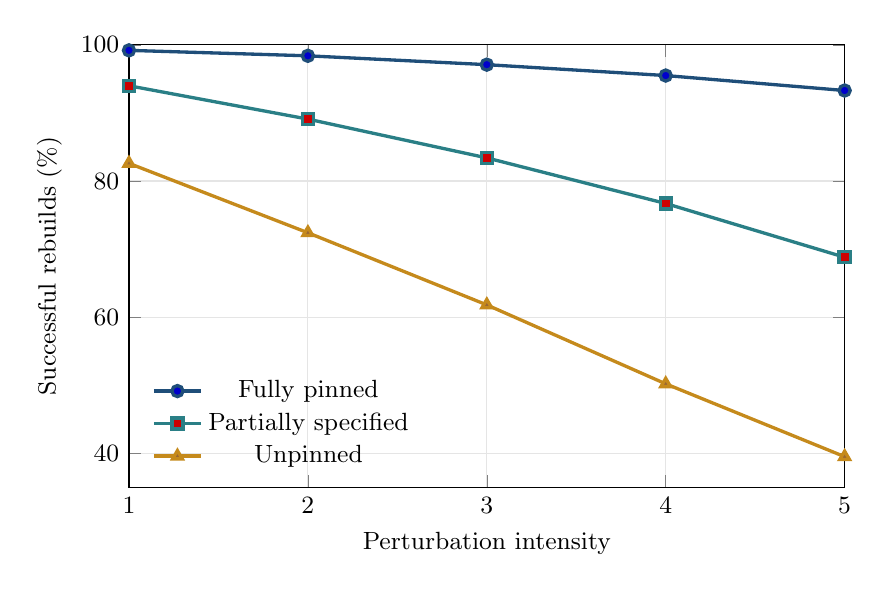
\begin{tikzpicture}
    \begin{axis}[
      width=0.88\textwidth,
      height=7.2cm,
      xmin=1,xmax=5,
      ymin=35,ymax=100,
      xtick={1,2,3,4,5},
      xlabel={Perturbation intensity},
      ylabel={Successful rebuilds (\%)},
      grid=major,
      grid style={gray!20},
      legend style={draw=none,fill=none,font=\small,at={(0.02,0.02)},anchor=south west},
      tick label style={font=\small},
      label style={font=\small}
    ]
      \addplot+[color=tandfblue,mark=*,very thick]
        coordinates {(1,99.2) (2,98.4) (3,97.1) (4,95.5) (5,93.3)};
      \addlegendentry{Fully pinned}
      \addplot+[color=tandfteal,mark=square*,very thick]
        coordinates {(1,94.0) (2,89.1) (3,83.4) (4,76.7) (5,68.8)};
      \addlegendentry{Partially specified}
      \addplot+[color=tandfgold,mark=triangle*,very thick]
        coordinates {(1,82.6) (2,72.4) (3,61.8) (4,50.2) (5,39.5)};
      \addlegendentry{Unpinned}
    \end{axis}
  \end{tikzpicture}
  \caption{Execution success across increasing environmental perturbation.
  Points are simulation means; connecting lines aid visual comparison.}
  \label{fig:success}
\end{figure}

\subsection{Complementary safeguards}

Environment capture and seed control affected different outcomes. Pinning
dependencies increased the probability that a pipeline completed, whereas seed
control primarily reduced dispersion among pipelines that did complete. In the
fully pinned condition, recording a seed reduced median numerical deviation from
1.3\% to 0.4\%. In the unpinned condition, the corresponding reduction was from
14.1\% to 11.8\%, because dependency changes dominated the remaining variation.
The interaction estimate was small and its interval included zero, supporting a
complementary rather than substitutive interpretation.

\section{Discussion}

The simulation illustrates why a successful rerun in the original environment
is an incomplete reproducibility test. Pipelines with fully captured environments
were substantially more resilient to dependency and system perturbations, and
explicit seed control improved numerical agreement within each environment
strategy. A compact evaluation should therefore report at least three elements:
execution success, numerical agreement, and the conditions under which both were
measured.

These findings align with calls to treat openness and reproducibility as
observable practices rather than aspirations \citep{nosek2015}. The proposed
framework adds a stress-testing layer: authors declare expected outputs, rebuild
the analysis under controlled changes, and report both failures and deviations.
This approach can be integrated into continuous-integration systems and repeated
when dependencies, data, or analysis code change.

\subsection{Limitations}

The study uses synthetic projects and stylized perturbations, so its numerical
estimates should not be interpreted as prevalence estimates for published
research. The simulated pipelines were also smaller than many production
workflows and did not represent specialized hardware, restricted data, or
interactive software. Empirical validation should sample real projects across
disciplines, define field-specific tolerances, and distinguish failures caused by
missing infrastructure from those caused by insufficient documentation.

\subsection{Implications for authors and reviewers}

For authors, the main practical implication is to preserve both the environment
and the sources of stochastic variation. For reviewers, a failed rebuild is most
informative when the submission records the attempted environment and the first
divergent stage. For journals, a short machine-readable manifest could accompany
the conventional data and code availability statements without imposing a
single software platform.

\section{Conclusion}

A robustness-first assessment reveals failure modes that a one-time successful
rerun cannot detect. In this simulation, version pinning protected execution,
while random-seed control improved agreement among completed rebuilds. Reporting
both outcomes offers a clearer and more actionable account of computational
reproducibility. The framework is deliberately lightweight and can be extended
to domain-specific data, software, and tolerance requirements.

\section*{Acknowledgements}

The authors thank the Northbridge Open Methods reading group for comments on an
earlier version of the reporting framework.

\section*{Disclosure statement}

The authors report no potential conflict of interest.

\section*{Funding}

This illustrative study received no external funding.

\section*{Data availability statement}

The manuscript describes a synthetic demonstration. All values required to
recreate its tables and figures are included directly in this source file. A
real submission should replace this statement with a persistent repository link
and any access conditions that apply to the underlying data.

\section*{Code availability statement}

The LaTeX source is self-contained and compiles with a standard TeX Live
distribution. No external analysis code is required for the illustrative
results. A research article should cite an archived release of its analysis code
and record the software environment used to produce the reported outputs.

\section*{Author contributions}

Maya Chen: conceptualization, methodology, writing---original draft, and
visualization. Daniel Okafor: formal analysis, validation, and writing---review
and editing. Sofia Alvarez: software, supervision, and writing---review and
editing. All authors approved the final manuscript.

\section*{Ethics statement}

This simulation study used no human participants, animals, personal data, or
clinical records; ethics approval and informed consent were therefore not
applicable.

\section*{Notes on contributors}

\textbf{Maya Chen} studies transparent computational methods and research
software sustainability. \textbf{Daniel Okafor} develops statistical methods
for evaluating complex data-analysis workflows. \textbf{Sofia Alvarez} leads
research-software engineering projects focused on durable and reusable scholarly
outputs.

\begin{thebibliography}{99}

\bibitem[Nosek et~al.(2015)Nosek, Alter, Banks, Borsboom, Bowman, Breckler,
  Buck, Chambers, Chin, Christensen, Contestabile, Dafoe, Eich, Freese, Glennerster,
  Goroff, Green, Hesse, Humphreys, Ishiyama, Karlan, Kraut, Lupia, Mabry, Madon,
  Malhotra, Mayo-Wilson, McNutt, Miguel, Paluck, Simonsohn, Soderberg, Spellman,
  Turitto, VandenBos, Vazire, Wagenmakers, Wilson, and Yarkoni]{nosek2015}
Nosek, B.~A., Alter, G., Banks, G.~C., et~al. (2015).
Promoting an open research culture.
\emph{Science}, 348(6242), 1422--1425.
\href{https://doi.org/10.1126/science.aab2374}{doi:10.1126/science.aab2374}.

\bibitem[Peng(2011)]{peng2011}
Peng, R.~D. (2011).
Reproducible research in computational science.
\emph{Science}, 334(6060), 1226--1227.
\href{https://doi.org/10.1126/science.1213847}{doi:10.1126/science.1213847}.

\bibitem[Sandve et~al.(2013)Sandve, Nekrutenko, Taylor, and Hovig]{sandve2013}
Sandve, G.~K., Nekrutenko, A., Taylor, J., and Hovig, E. (2013).
Ten simple rules for reproducible computational research.
\emph{PLoS Computational Biology}, 9(10), e1003285.
\href{https://doi.org/10.1371/journal.pcbi.1003285}{doi:10.1371/journal.pcbi.1003285}.

\bibitem[Stodden et~al.(2016)Stodden, McNutt, Bailey, Deelman, Gil, Hanson,
  Heroux, Ioannidis, and Taufer]{stodden2016}
Stodden, V., McNutt, M., Bailey, D.~H., Deelman, E., Gil, Y., Hanson, B.,
Heroux, M.~A., Ioannidis, J.~P.~A., and Taufer, M. (2016).
Enhancing reproducibility for computational methods.
\emph{Science}, 354(6317), 1240--1241.
\href{https://doi.org/10.1126/science.aah6168}{doi:10.1126/science.aah6168}.

\bibitem[Wilkinson et~al.(2016)Wilkinson, Dumontier, Aalbersberg, Appleton,
  Axton, Baak, Blomberg, Boiten, da~Silva~Santos, Bourne, Bouwman, Brookes,
  Clark, Crosas, Dillo, Dumon, Edmunds, Evelo, Finkers, Gonzalez-Beltran, Gray,
  Groth, Goble, Grethe, Heringa, 't~Hoen, Hooft, Kuhn, Kok, Kok, Lusher,
  Martone, Mons, Packer, Persson, Rocca-Serra, Roos, van~Schaik, Sansone,
  Schultes, Sengstag, Slater, Strawn, Swertz, Thompson, van~der~Lei,
  van~Mulligen, Velterop, Waagmeester, Wittenburg, Wolstencroft, Zhao, and
  Mons]{wilkinson2016}
Wilkinson, M.~D., Dumontier, M., Aalbersberg, I.~J., et~al. (2016).
The FAIR guiding principles for scientific data management and stewardship.
\emph{Scientific Data}, 3, 160018.
\href{https://doi.org/10.1038/sdata.2016.18}{doi:10.1038/sdata.2016.18}.

\end{thebibliography}

\appendix
\section{Minimal robustness-reporting checklist}

Table~\ref{tab:checklist} provides a compact checklist that can accompany the
main manuscript or supplementary material.

\begin{table}[htbp]
  \centering
  \caption{Suggested information for a computational robustness report.}
  \label{tab:checklist}
  \begin{singlespace}
  \small
  \begin{tabularx}{\textwidth}{@{}>{\bfseries}p{0.25\textwidth}X@{}}
    \toprule
    Item & Information to report \\
    \midrule
    Reference environment & Operating system, language runtime, direct and
      transitive dependencies, and hardware requirements. \\
    Declared outputs & Files, tables, figures, or numerical estimates that
      constitute a successful run. \\
    Perturbations & Dependency updates, system changes, randomization, and the
      rationale for their tested ranges. \\
    Agreement criterion & Numerical or qualitative tolerance used to judge a
      rebuilt result against its reference. \\
    Failure record & Stage of failure, diagnostic message, attempted remedy,
      and whether the failure is deterministic. \\
    Preservation & Persistent identifiers for data, code, environment files,
      and the exact release evaluated in the manuscript. \\
    \bottomrule
  \end{tabularx}
  \end{singlespace}
\end{table}

\end{document}
